\documentclass[12pt, letterpaper]{article}

\usepackage[utf8]{inputenc}  % Basic character encoding
\usepackage{amsmath}         % For mathematical  formulas
\usepackage{amssymb}         % Provides an extended symbol collection.
\usepackage{pgfplots}        % For plotting

\setcounter{secnumdepth}{0} % sections are level 1

% personal data
\title{Pre-Calculus from Zero}
\author{Basic Pre-Calculus Topics}
\date{Dec 2017}

% End of preamble
\begin{document}

\maketitle

\section{Introduction}

The Pythagorean theorem $x^2 + y^2 = z^2$ was proved to be invalid for other
exponents. Meaning the next equation has no integer solutions:

$$x^n+ y^n = z^n$$
\section{Arithmetic}
\section{Algebra}
\section{Sets}

In mathematics, a set is a collection of distinct objects. A set is also itself
an object. For example, the numbers 2, 4, and 6 are distinct objects
when considered separately, but when they are considered collectively they form
a single set of size three, written {2,4,6}.
\\

\noindent$\mathbb{P}$, denoting the set of all primes:
$\mathbb{P}$ = (2, 3, 5, 7, 11, 13, 17, ...)
\\\\
A prime number is a natural number greater than 1 that has no positive
divisors other than 1 and itself.
\\

\noindent$\mathbb{N}$, denoting the set of all natural numbers: $\mathbb{N}$ =
(0, 1, 2, 3, ...)
\\\\
The natural numbers are those used for counting.
\\

\noindent$\mathbb{Z}$, denoting the set of all integers: $\mathbb{Z}$ =
(..., -2, -1, 0, 1, 2, ...)
\\\\
An integer is a number that can be written without a fractional component.
For example, 22, 6, 0 and -2048 are integers,
while 4.75, 5$\frac{1}{2}$ and $\sqrt{2}$ are not.
\\

\noindent$\mathbb{Q}$, denoting the set of all rational numbers: $\mathbb{Q}$ =
(a/b : a, b $\in$ Z, b $\neq$ 0)
\\\\
A rational number is any number that can be expressed as the quotient or
fraction p/q of two integers, a numerator p and a non-zero denominator q.
\\

\noindent$\mathbb{R}$, denoting the set of all real numbers.
\\\\
A real number is a value that represents a quantity along a line.
\\

\section{Rectangular Coordinates}

Just as you can represent real numbers by points on a real number line, you can
represent ordered pairs of real numbers by points in a plane called the
rectangular coordinate system, or the Cartesian plane, named after the French
mathematician René Descartes (1596–1650).
\\
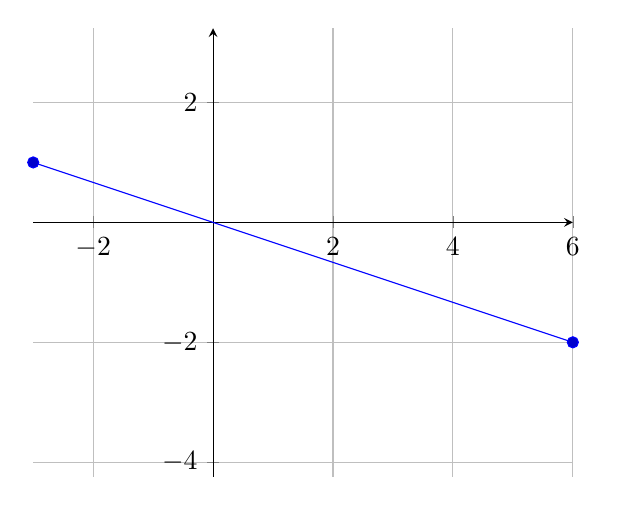
\begin{tikzpicture}
\begin{axis}[axis lines=middle,axis equal,grid=both]
\addplot coordinates{(-3,1) (6,-2)};
\end{axis}
\end{tikzpicture}

\section{Factoring}

The GCF (greatest common factor) of two or more monomials is the product of all 
their common prime factors. For example, the GCF of $6x$ and $4x^2$ is $2x$.

For example, to factor $-\frac{3}{5}z^3 - 6z^2$, we would first get a common
denominator and factor as: 
\[ -\frac{3}{5}z^3 - 6z^2 = \frac{-3z^3 - 30z^2}{5} =
\frac{-3z^2(z + 10)}{5} = -\frac{3z^2(z + 10)}{5}\]

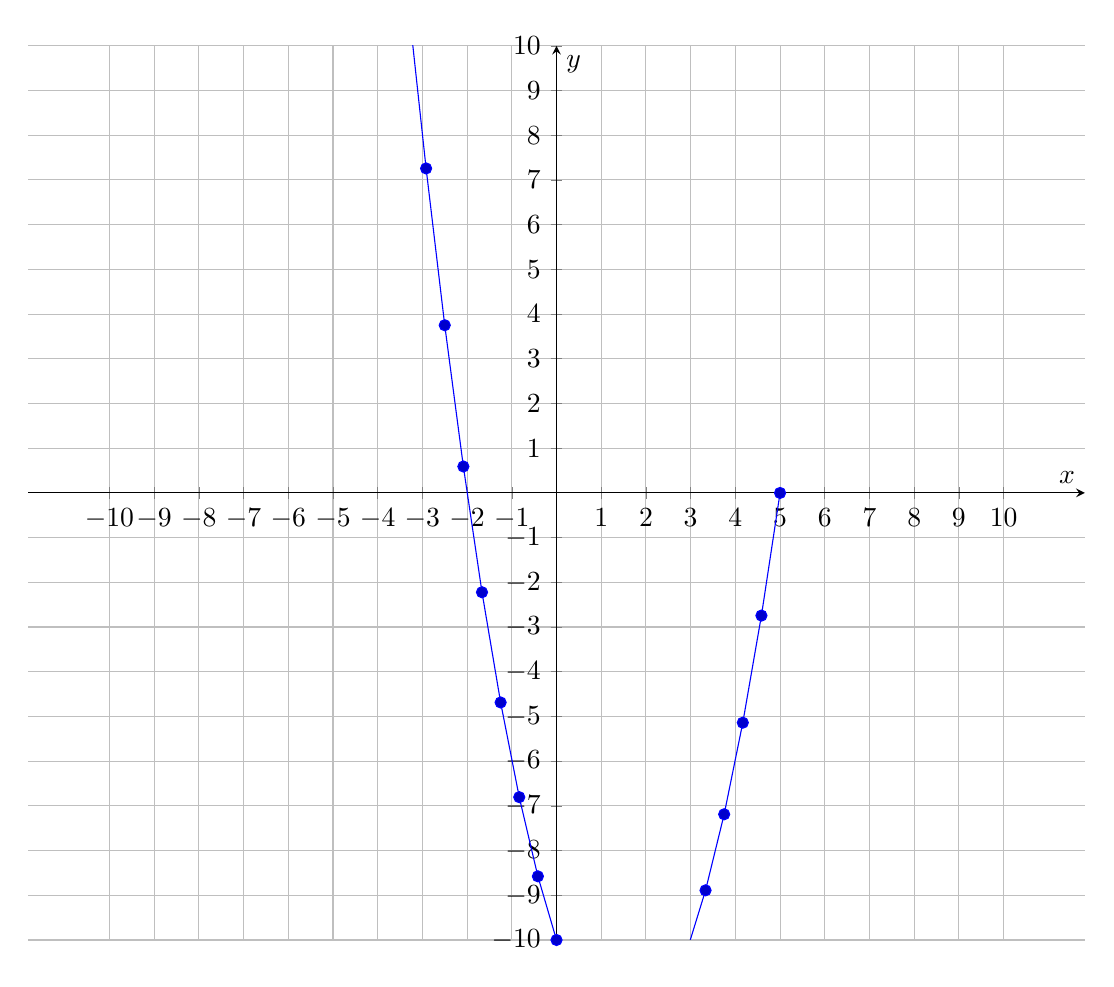
\begin{tikzpicture}[baseline]
\begin{axis}[
axis y line=center,
axis x line=middle,
axis equal,
grid=both,
xmax=10,xmin=-10,
ymin=-10,ymax=10,
xlabel=$x$,ylabel=$y$,
xtick={-10,...,10},
ytick={-10,...,10},
width=15cm,
anchor=center,
]
\addplot {x^2-3*x-10} ;
\end{axis}
\end{tikzpicture}

\section{Polynomial Functions}

Info here. Add some information on the subject above. 

\section{Rational Functions}

Info here. Add some information on the subject above. 

\section{Exponential Functions}

Info here. Add some information on the subject above. 

\section{Logarythmic Functions}

Info here. Add some information on the subject above. 

\section{Trigonometry}

Info here. Add some information on the subject above. 

\section{Analytic Trigonoetry}

Info here. Add some information on the subject above. 

\end{document}
